\chapter{Diagnostic Models}

This section analyses storage systems (also known as warehousing systems). The scientific field analysing storage system is warehouse science ~\cite{Bartholdi2017}. This topic is profoundly important in the management of a supply chain since warehouses are the first source of inefficiencies in a supply chain. The assignment of a proper inventory level in the warehouses of a supply chain network is the first step to smooth the flows and improve the operations of the entire chain.\par

Warehouses work as decoupling points between other supply chain nodes ~\cite{Aguezzoul2014, Selviaridis2007}. Their role is unavoidable since they enhance the flexibility of the entire supply chain by separating the demand and the production rates. We often hear of \textit{zero inventory} as the central paradigm of lean thinking. In truth, it is impossible to build a supply chain without inventory. Contrarily, it is absolutely possible, and always recommendable, to design supply chain able to keep the inventory levels under control (that is the real meaning of the \textit{zero inventory} philosophy). \par

Nevertheless, the stock is a cost with, or without the control on the level of the inventory. Warehouses do not add any value to the product, but they always lead to costs. For this reason, it is necessary to pay close attention to the design and control of warehouses in order to avoid inefficiencies.\par

Warehouses retain all the ingredients for a data-driven approach. Operations within warehouses are pretty repetitive, and even the warehouse layout is easy-to-model; it is composed of many standard blocks working the same way. Besides, for traceability reasons, warehouses produce tons of data to keep track of put-away, picking operations, and inventory positions.\par

This chapter focuses on the definition of the keywords and key entities extending the ontology of Chapter \ref{chap_InformationFramework} to storage nodes. After that, we introduce the diagnostic framework for production nodes using a relational data structure and a dashboard of KPIs. A non-relational data structure is proposed as well, to enhance data-driven features by combining the information sources of multiple storage systems.\par

Chapter \ref{chapWhControl} focuses on data- and model-driven methods to control a storage node, while chapter \ref{chapWhDesign} does the same focusing on the design methods.

\section{Ontology} \label{secOntology_wh}
Section \ref{chap_InformationFramework} introduces the general ontology of this book. This paragraph develops that ontology by applying its keys and metrics to a warehouse system.

\subsubsection{Entities}
We identify the following entities:\par
\textbf{Part} ($i$): it is a storage unit, better known as a stock keeping unit (SKU). An SKU is usually:
\begin{itemize}
    \item a part, i.e. a single product;
    \item a carton, i.e. a (secondary) package, containing many parts, or 
    \item a pallet, i.e. a (tertiary) package, containing many cartons.
\end{itemize}
\par

\textbf{Processing node} ($j$): it is a storage location. Each area able to host one or more SKUs is a processing node of the storage system. \par

\textbf{Edge} ($j,k$): paths connecting the storage locations (the aisles of the warehouse) are the edges. Generally, aisles can be travelled:
\begin{itemize}
    \item traversal (using a single direction);
    \item teturn (using both the directions).
\end{itemize}
Traversal policy implies that the graph of the storage system is directed. Otherwise, return policy implies an undirected graph.
\par

\textbf{Vehicle} ($v$): a vehicle is any unit able to travel on edges and load or unload parts (e.g. a forklift). \par

\textbf{Consumable} ($s$): the energy to feed the vehicles, and the resources of a storage system.\par

\textbf{Route} ($e$): the routes in a storage system are the set of edges travelled in sequence by a vehicle to complete a put-away or picking job. Routes are usually not predefined and can continuously change depending on the set of orders. \par

\textbf{Order} ($o$): it is a set of products to put away or pick received by the customer \par

\textbf{Job} ($b$): it is the sequence of locations to visit and the quantity of SKUs to move to complete an order. A picking/put-away list is a job. \par

\textbf{System network}: the graph $G(V,A)$ of nodes $j\in V$ and edges $\left(j,k\right)\in A$ composing the warehouse system.

\subsubsection{Metrics}
We identify the following metrics to assess the performances of a processing node $j$.\par

\textbf{Throughput} ($TH_{j}$): the put-away or picking rate of a set of locations. (parts per hour).\par

\textbf{Work in process} ($WIP_{j}$): it is the number of parts stored in a location $j$.\par

\textbf{Work in process} ($WIP_{jk}$): it is the number of parts being transported by a vehicle $v$. \par

\textbf{Capacity} ($C_j$): it is the maximum storage capacity of a storage location $j$, usually measured in quantity or volume ($dm^3$).\par

\textbf{Capacity} ($C_v$): it is the maximum number of part transportable by a vehicle $v$ at the same time. \par

\textbf{Utilisation} ($U_j$): it is the average saturation of the space of a storage location. \par

\textbf{Utilisation} ($U_v$): it is the average fraction of non-empty space on a vehicle. \par

\textbf{Lead time} ($LT_e$): it is the time allocated to perform a route (i.e. to complete a picking or put-away list). \par

\textbf{Cycle time} ($CT_e$): it is the average time from the receipt of an order to the completion of the associated picking list (job). \par

\textbf{Service level} ($SL_e$): $Prob\{cycle\ time\le lead\ time\}$

\subsubsection{Information functions}

Finally, we define the three information functions introduced \ref{secInfoFramework}: movements $M$ are referred to put-away (IN) and picks (OUT) of SKUs to or from a storage location $j$; the inventory $I$ is referred to the number of SKUs stored in a storage location $j$. The productivity $P$ refers to the inbound and outbound throughput of a set of locations. Usually, a set contains locations close to each other, depending on the warehouse technology (e.g. manual or automated) offering a different $TH_j$ and with different productivity patterns. Table \ref{tab_information_function_wh} summarises the definition of the three functions in a storage system.

% INSERT tab_information_function_wh
\begin{figure}[hbt!]
\centering
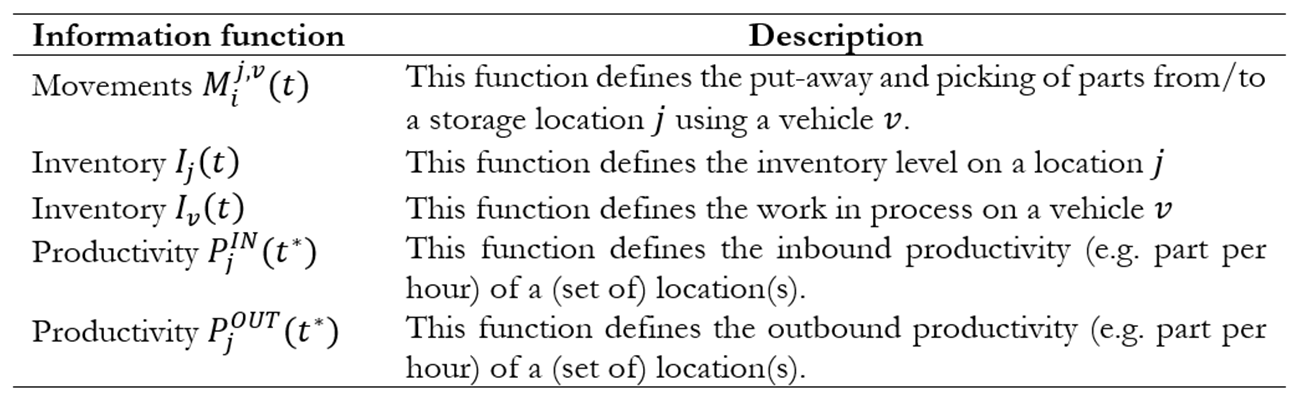
\includegraphics[width=1\textwidth]{SectionWarehouses/diagnsticModels_figures/tab_information_function_wh.png}
\captionsetup{type=table}
\caption{Definition of the information functions of a storage system.}
\label{tab_information_function_wh}
\end{figure}


\section{Data Structure}
This paragraph introduces an ER model to describe the operations of a storage system. Warehouses operations are similar for different nodes and enterprises, and despite their level of automation, it is possible to define a rigid model able to identify the aspects of value from a logistics perspective. For this reason, the relational database infrastructures are still the most widely used in the industry ~\cite{Accorsi2014}. 

\subsection{A relational model for warehousing systems}
The ER model has a table for each of the relevant aspects of a storage system:
\begin{enumerate}
    \item the SKUs;
    \item the storage locations;
    \item the vehicles;
    \item the inventory position;
    \item the movements.
\end{enumerate}

\subsubsection{SKUs}
The SKUs table contains all the information from the SKU master file. The features of the SKUs are relevant to identify the proper storage area for each SKU, depending on its dimensions, weight, volume, inflammability, shelflife, and many other industry-oriented features. For these reasons, the SKU table identifies:

\begin{itemize}
    \item the id of the item;
    \item the description of the item;
    \item the category of the item (e.g. the commercial category);
    \item the id of the product family of the item;
    \item the temperature profile of the item (if any);
    \item the production route of the item (if any);
    \item the package route of the item (if any);
    \item the volume and weight of the item;
    \item the size (i.e. length, height, width) of the item;
    \item the supplier of the item.

\end{itemize}

The description, size volume and weight are the most important information to design the storage system and to identify the proper location of the item. Other information as the supplier, the category, the product family may be of interest to place similar items in different zones of the storage system. The production and the package flow are important information for the picker who has to place the item on the correct flow (e.g. in a packing area) before the shipping.

\subsubsection{Storage locations}

Storage locations are the areas where each single SKU is stored and waits to be picked. Many information is tracked for each location to enhance the traceability and to speed up the put-away and picking process (in particular, the search of a specific location). For each location, this table keeps track of:

\begin{itemize}
    \item the id of the storage system (i.e. the building);
    \item the id of the logical warehouse (i.e. a subset of locations that are logically but not necessarily physically separated by the others);
    \item the id of the location;
    \item the coordinate of the aisle which serves the location ($x$ coordinate);
    \item the coordinates of the location ($x,y,z$ coordinates);
    \item the number of the rack;
    \item the number of the bay;
    \item the number of the level;
    \item the id of the area where the location is placed;
    \item the category of the vehicle serving the location;
    \item the type of the package (part/carton/pallet) stored in the location.

\end{itemize}

This information is beneficial to analyse the flows generated by the warehouse on its plant layout. Nevertheless, the majority of the warehouse management systems (WMS) does not keep track of the physical coordinates of storage locations, creating a significant lack of data for warehouse control and improvement.

\subsubsection{Vehicles}
The vehicles table identifies the macro category of vehicles handling SKUs within a warehouse. A non-exhaustive list comprises:

\begin{itemize}
    \item manual operator (i.e. walking through aisles and shelves);
    \item forklift serving racks;
    \item forklift serving floor stack;
    \item man-on-board picking vehicle;
    \item vertical warehouse (e.g. Modula);
    \item miniload;
    \item automated storage \& retrieval system (AR/RS).

\end{itemize}

\subsubsection{Inventory}
This table defines the inventory level of each storage location at a specific date defining the quantity of the item codes stored in that location. Its attributes are:

\begin{itemize}
    \item the id of the storage system (i.e. the building) inherited from the table locations;
    \item the id of the logical warehouse (i.e. a subset of locations that are logically but not necessarily physically separated by the others) inherited from the table locations;
    \item the id of the location inherited from the table locations;
    \item the id of the item inherited from the SKU table;
    \item the timestamp when the inventory is recorded;
    \item the number of parts of the item code above stored in the location.

\end{itemize}

The inventory information defines the state of a storage location at a precise timestamp.

\subsubsection{Movements}
The movements table tracks each movement, i.e. put-away or picking activity modifying the state of a storage location (i.e. its storage level). The table records the following attributes:

\begin{itemize}
    \item the id of the storage system (i.e. the building) inherited from the table locations;
    \item the id of the logical warehouse (i.e. a subset of locations that are logically but not necessarily physically separated by the others) inherited from the table locations;
    \item the id of the location inherited from the table locations;
    \item the id of the item inherited from the SKU table;
    \item the timestamp when the movement is recorded;
    \item the id of the order;
    \item the quantity picked or put away;
    \item the id of the picking/put-away mission;
    \item the sign of the movement (e.g. '+' for put-away and '-' for picking)
    \item the type of the order;
    \item the id of the picking operator/vehicle;
    \item the id of the package associated with the SKU.

\end{itemize}

Figure \ref{fig_ER_wh} presents the relational model linking all these tables by the definition of relationship and integrity constraints between entities.

% INSERT fig_ER_wh
\begin{figure}[hbt!]
\centering
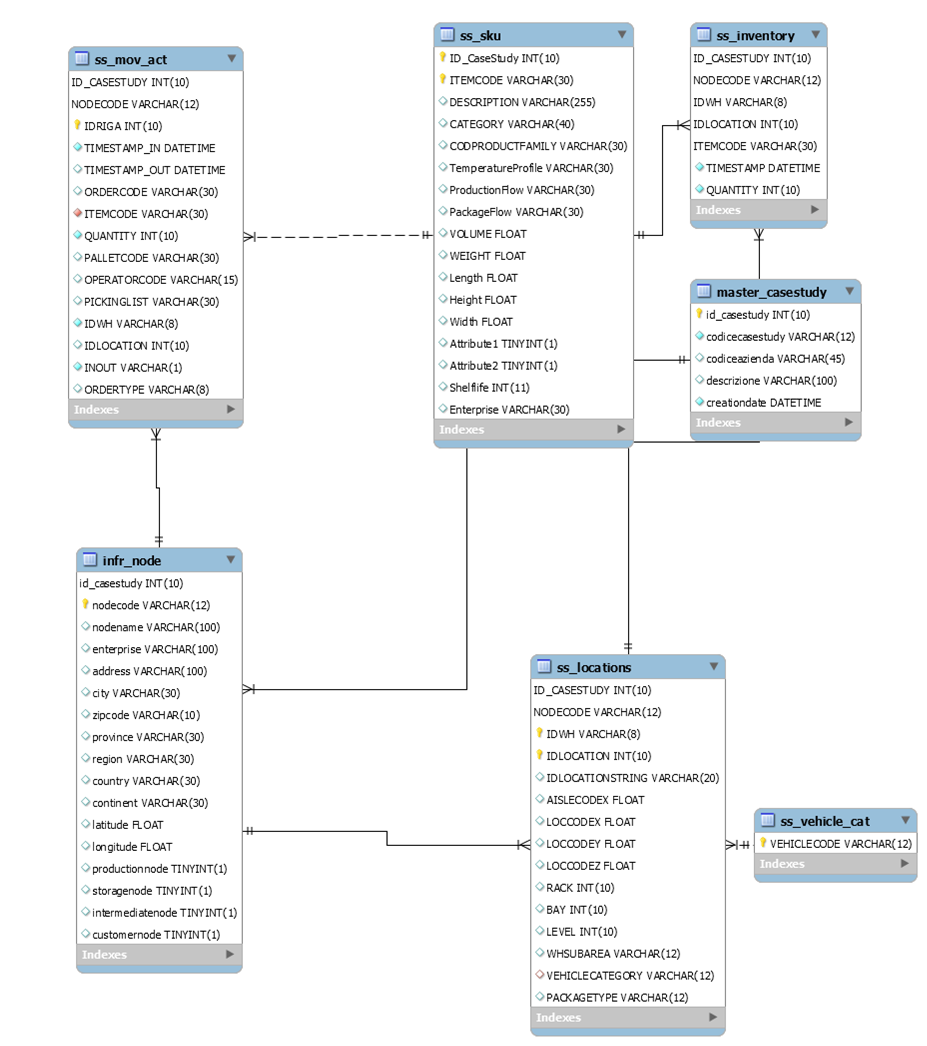
\includegraphics[width=1\textwidth]{SectionWarehouses/diagnsticModels_figures/fig_ER.png}
\captionsetup{type=figure}
\caption{ER-model for storage systems.}
\label{fig_ER_wh}
\end{figure}

\subsection{A non-relational model for warehousing systems} \label{secNonRelStructWh}

ER databases are the most used in the design of the WMS. Nevertheless, non-relational structures allow flexibility and easiness of use with benefits applied to the field of warehousing science. In particular, traditional WMS does not store information on the layout coordinates of the storage locations. In addition, many locations are virtual and only exists in the WMS to provide relational integrity without any physical relevance. \par

An important feature to control a storage system is the possibility to measure the distance between storage locations. While dealing with an ER structure, it is possible to define a block-layout identifying:

\begin{itemize}
    \item the input and output points;
    \item the presence of traversal aisles;
    \item a modular distance between storage locations of the same aisle;
    \item a modular distance between aisles.
\end{itemize}

Figure \ref{fig_layout_wh} identifies the layout, and its coordinates identified by these features. The coordinates are identified by using the letter $a$ for the aisles, the letter $r$ for the racks, and the letter $t$ for the traversal aisles.

% INSERT fig_layout_wh
\begin{figure}[hbt!]
\centering
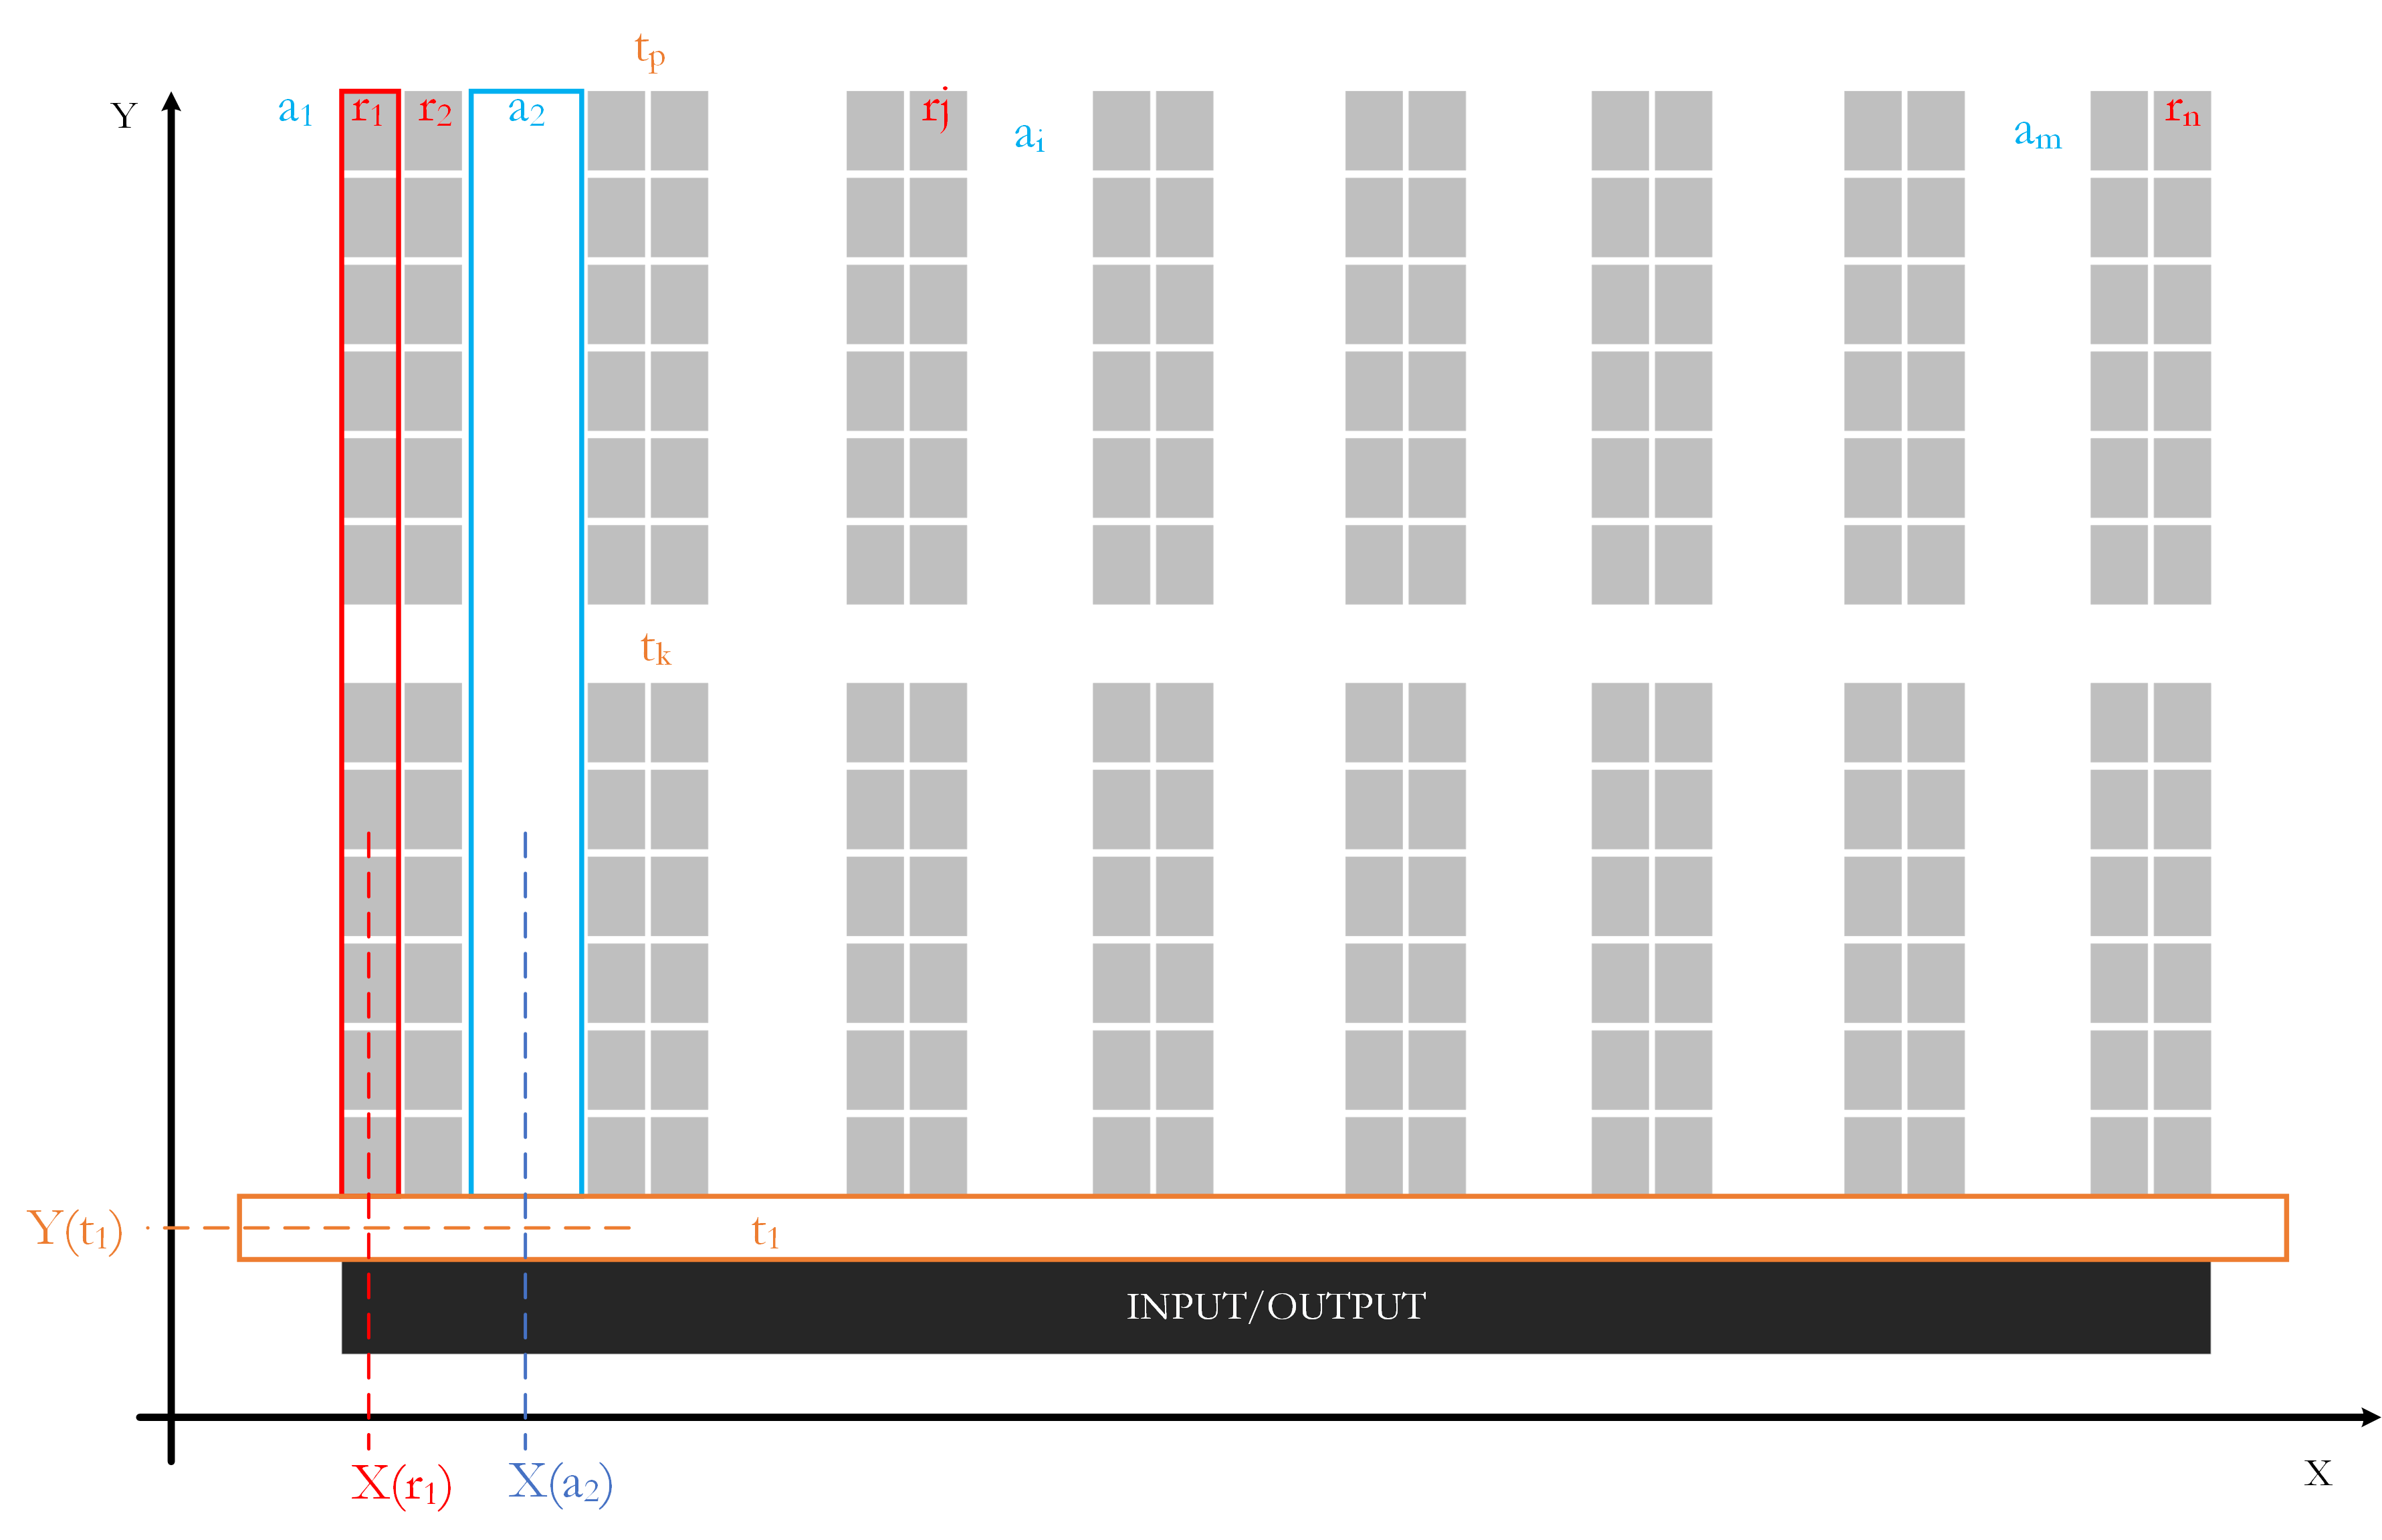
\includegraphics[width=1\textwidth]{SectionWarehouses/diagnsticModels_figures/fig_layout.png}
\captionsetup{type=figure}
\caption{Warehouse layout model.}
\label{fig_layout_wh}
\end{figure}

Unluckily, the application of modular distances does not always correctly represent the distances within a storage system, adding an avoidable bias. There can be multiple storage blocks within the same warehouses using different technologies, or different storage areas whose distances are poorly represented by this modular pattern. To overcome this limitation, we aim at defining a graph $G(V,A)$ with a vertex $j\in V$ for each  storage location, and a set of arcs $\left(i,j\right)\in A$ representing the available connections with their distance. A non-relational structure is the natural tool to both contain all the information of the relational model, and to save the graph $G$ to enhance warehouse design and control. We introduce the collections and attributes of the non-relational data structure first. Then we illustrate a method to define the warehouse graph. \par

The non-relational data structure consists of five collections: \textit{parts}, \textit{storage locations}, \textit{movements}, \textit{inventory} and \textit{graph}. For each collection, a minimal number of attributes defines the minimal viable model (MVM) with the essential information to map the operations of a storage system. \par

The collection \textit{parts}, is similar to the table SKU of the relational model. It stores the information from the SKUs master file of the storage system. The id of each SKU is the only attribute necessary to have an MVM. \par

The collection \textit{storage locations} records information on the storage location of the warehouse. The id of the storage location is the only attribute necessary to define the MVM. Additional attributes can be recorded as:

\begin{itemize}
    \item the coordinates of the location; 
    \item the coordinates of the aisle; 
    \item the list of the type of vehicles serving the location; 
    \item the available capacity of the location; 
    \item the logical warehouse containing the location;
    \item the inventory function of the storage location.
\end{itemize}

The collection \textit{movements} records all the activities performed in the warehouse. The necessary attributes of the MVM are:
\begin{itemize}
    \item the timestamp;
    \item the id of the part; 
    \item the id of the storage location;
    \item the id of the order;
    \item the quantity;
    \item the sign (i.e. “+” or “-“). 
\end{itemize}

Other attributes that can be recorded are:
\begin{itemize}
    \item the id of the picking list; 
    \item the id of the operator; 
    \item the weight of the movement; 
    \item the volume of the movement; 
    \item the destination of the movement. 
\end{itemize}

The collection \textit{inventory} stores observation of the inventory position of the warehouse. The MVM is composed by:
\begin{itemize}
    \item the timestamp;
    \item the id of the part; 
    \item the id of the location;
    \item the observed quantity. 
\end{itemize}

Figure \ref{fig_MVM_wh} uses the unified modelling language (UML) to represent the MVM of the non-relational data structure of a storage system.

% INSERT fig_MVM_wh
\begin{figure}[hbt!]
\centering
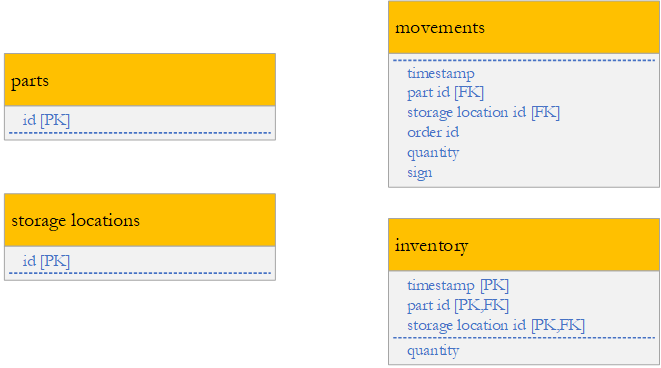
\includegraphics[width=0.8\textwidth]{SectionWarehouses/diagnsticModels_figures/fig_MVM.png}
\captionsetup{type=figure}
\caption{Diagram in UML notation of the minimum viable model for a non-relational structure of a storage system.}
\label{fig_MVM_wh}
\end{figure}


Finally, a collection graph stores a single graph object $G(V,E)$, representing the graph of the storage system, defined using a standard procedure \footnote{The source code to generate the graph of a storage system is available \href{https://github.com/aletuf93/logproj/blob/master/logproj/P6_placementProblem/warehouse_graph_definition.py}{here}.}. Algorithm \ref{algo_whGraphDefinition} illustrates this procedure appliable to any warehouse dataset. It aims at defining a graph with edges and vertices associated with all the storage locations recorded in the storage location collection. First, the procedure defines the set of vertices $V$ by considering all the coordinates of the storage locations projected onto the aisles that serve them. Then a set of edges $E$ is created to connect all these vertices virtualising the path of the aisles of the warehouse. Missing values (e.g. missing coordinates in the storage location collections) are replaced by using linear interpolation between the known values.


% Algorithm wh graph definition
\begin{algorithm}[H]
\DontPrintSemicolon
\SetAlgoLined


Import storage locations $s \in S$\;
Import I/O locations $f \in F$\;
Set $L={S \bigcup F}$\;
Consider $L_a$, aisle coordinate for each storage location\;
Set $V={L_{a}(x,y)}$\;
Clean the coordinates $L_a$ with linear interpolation of missing values\;
{\If {$F==\emptyset$}
    {
    Define a I/O point in (
    $\frac{max\{L_a(y)\} - min\{L_a(y)\}}{2}$,$min\{L_a(x)\}$
    )\;
    }
}
Map fake locations with coordinates in $F$\;
Set $E=\emptyset$\;
$E=E\bigcup \{$vertical edges connecting aligned coordinates$\}$\;
$E=E\bigcup \{$horizontal on the front and back of the warehouse$\}$\;
$E=E\bigcup \{$edges connecting the I/O points to the closest node$\}$\;
\caption{Definition of the warehouse graph.}
\label{algo_whGraphDefinition}   
\end{algorithm}

\section{Decision Patterns}
This section aims at defining the set of decision problems for the design and control of a storage system, using the decision patterns identified in \ref{secDecisionPatterns}. Problems are classified into:

\begin{enumerate}
    \item Warehouse design problems, dealing with the design and placement of the physical entities of a storage system;
    \item Warehouse control problems, dealing with the assessment and improvement of the performance of an existing storage system.
\end{enumerate}

Different methodologies allow getting feasible solutions to these problems \cite{Cormier1992, Gray1992, Manzini2015, VandenBerg1999a}. Table \ref{tab_problems_wh} illustrates the entities and their definition according to the ontology in \ref{secOntology} involved in each decision pattern. 


% INSERT tab_problems_wh
\begin{landscape}
\thispagestyle{empty}
\begin{figure}[hbt!]
\centering
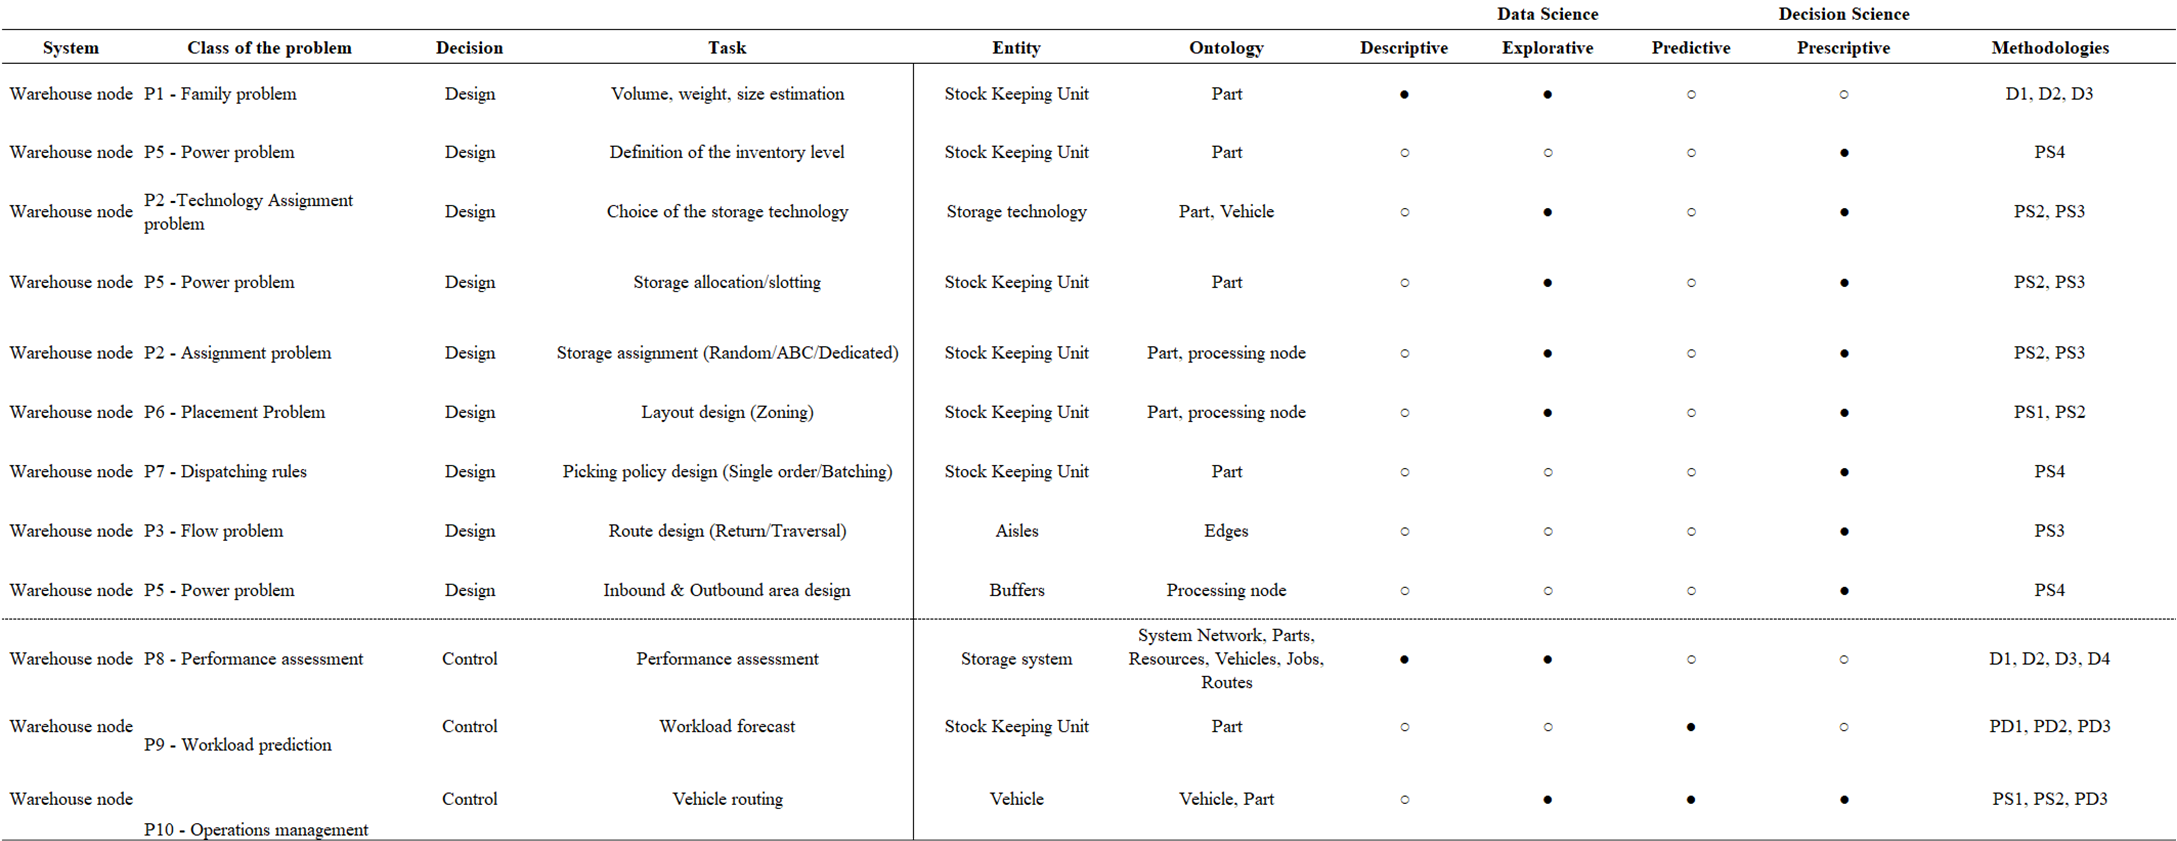
\includegraphics[width=1.5\textwidth]{SectionWarehouses/diagnsticModels_figures/tab_problems_wh.png}
\captionsetup{type=table}
\caption{Decision problems classification in a storage system.}
\label{tab_problems_wh}
\end{figure}
\end{landscape}


Twelve decision problems are identified in the design and control of a storage node:
\begin{enumerate}
    \item Volume, weight, size estimation; it involves the definition or estimation of the attributes of an SKU.
    \item Choice of the storage system; it involves the definition of an adequate set of vehicles to serve the storage needs.
    \item Forward-reserve design; it involves the design of a reserve area (on the upper levels of a storage system) serving a fast pick area on the floor.
    \item Storage allocation; it involves the design of the level of inventories on the fast-pick and reserve area.
    \item Storage assignment; it involves the assignment of SKUs to storage locations.
    \item Layout design; it involves the design of the areas (i.e. the zones) of the storage system.
    \item Picking policy design; it involves the definition of the picking policies (e.g. single-order vs. batching and sorting).
    \item Route design; it involves the definition of the direction allowable for each aisle (i.e. return or traversal)
    \item Inbound and outbound area design; it involves the definition of the amount of space dedicated to inbound and outbound operations
    \item Performance assessment (control); it involves the measurement of the performance of a storage system.
    \item Workload forecast (control); it involves the prediction of the workload and workforce needed to perform the operation in the short-, mid- or long-term
    \item Vehicle routing (control); it involves the definition of the picking/put-away lists and their assignment to vehicles.

\end{enumerate}

Besides, Table \ref{tab_problems_wh} specifies which data science technique results adequate to propose a solution to the problem. While descriptive and prescriptive techniques are preferred for control problems, explorative and prescriptive techniques result adequate when dealing with design problems. Chapters \ref{chapWhControl} and \ref{chapWhDesign} illustrate these techniques in details.





%\clearpage
\bibliographystyle{ieeetr}
\bibliography{SectionWarehouses/diagnosticModels_ref}